\documentclass[a4paper]{article}
\usepackage[utf8]{inputenc}
\usepackage[spanish, es-tabla, es-noshorthands]{babel}
\usepackage[table,xcdraw]{xcolor}
\usepackage[a4paper, footnotesep = 1cm, width=20cm, top=2.5cm, height=25cm, textwidth=18cm, textheight=25cm]{geometry}
%\geometry{showframe}

\usepackage{tikz}
\usepackage{amsmath}
\usepackage{amsfonts}
\usepackage{amssymb}
\usepackage{float}
\usepackage{graphicx}
\usepackage{caption}
\usepackage{subcaption}
\usepackage{multicol}
\usepackage{multirow}
\setlength{\doublerulesep}{\arrayrulewidth}
\usepackage{booktabs}
\usepackage{mathrsfs,amsmath}
\usepackage{hyperref}
\hypersetup{
    colorlinks=true,
    linkcolor=blue,
    filecolor=magenta,      
    urlcolor=blue,
    citecolor=blue,    
}

\newcommand{\quotes}[1]{``#1''}
\usepackage{array}
\newcolumntype{C}[1]{>{\centering\let\newline\\\arraybackslash\hspace{0pt}}m{#1}}
\usepackage[american]{circuitikz}
\usetikzlibrary{calc}
\usepackage{fancyhdr}
\usepackage{units} 

\graphicspath{./Imagenes}

\pagestyle{fancy}
\fancyhf{}
\lhead{22.05 ASSD}
\rhead{Mechoulam, Lambertucci, Rodriguez, Londero}
\rfoot{Página \thepage}

\begin{document}

%%%%%%%%%%%%%%%%%%%%%%%%%
%		Caratula		%
%%%%%%%%%%%%%%%%%%%%%%%%%

\begin{titlepage}
\newcommand{\HRule}{\rule{\linewidth}{0.5mm}}
\center
\mbox{\textsc{\LARGE \bfseries {Instituto Tecnológico de Buenos Aires}}}\\[1.5cm]
\textsc{\Large 22.05 Análisis de Señales y Sistemas Digitales}\\[0.5cm]


\HRule \\[0.6cm]
{ \Huge \bfseries Trabajo práctico N$^{\circ}$2}\\[0.4cm] 
\HRule \\[1.5cm]


{\large

\emph{Grupo 3}\\
\vspace{3px}

\begin{tabular}{lr} 	
\textsc{Mechoulam}, Alan  &  58438\\
\textsc{Lambertucci}, Guido Enrique  & 58009 \\
\textsc{Rodriguez Turco}, Martín Sebastian  & 56629 \\
\textsc{Londero Bonaparte}, Tomás Guillermo  & 58150 \\
\end{tabular}

\vspace{20px}

\emph{Profesores}\\
Jacoby, Daniel Andres\\
Belaustegui Goitia, Carlos F.\\
Iribarren, Rodrigo Iñaki\\
\vspace{3px}
%\textsc{} \\	

\vspace{100px}

\begin{tabular}{ll}

Presentado: & 15/05/20\\

\end{tabular}

}

\vfill

\end{titlepage}


%%%%%%%%%%%%%%%%%%%%%
%		Indice		%
%%%%%%%%%%%%%%%%%%%%%

%\tableofcontents
%\newpage

%%%%%%%%%%%%%%%%%%%%%
%		Informe		%
%%%%%%%%%%%%%%%%%%%%%
\begin{center}
	\Large{\textcolor{red}{\textbf{EN ROJO PONGO LO QUE HAY QUE HACER. NO BORRARLO HASTA NO TERMINARLO. RESPETAR FORMATOS.}} \textcolor{blue}{EN AZUL IDEAS DE QUE DESARROLLAR.}}
\end{center}

\textbf{\textit{En el siguiente trabajo se presenta el estudio, investigación y análisis de un proceso de seguimiento del movimiento de un objeto mediante una cámara, siendo conocida su posición inicial.}}

\textcolor{red}{\textbf{\textit{Resumen: falta mencionar ensayos y resultados.}}}

\section{Introducción}
Una imagen puede ser interpretada como una función bidimenional $f\left( x, y\right)$, donde tanto $x$ como $y$ representan en un plano el epacio visualizado, mientras que la misma función $f\left( x, y\right)$ es la instensidad de la imagen bajo un punto dado. Cuando $x$, $y$ y $f\left( x, y\right)$ son valores cuantizados y discretizados, la imagen se transforma en una imagen digital.
	 	
El procesamiento de dichas se define como el conjunto de técnicas aplicadas a estas imágenes, con el objetivo extraer información de ellas. Estas actividades cubren un campo que abarca un sin fin de aplicaciones, ya que se vale de maquinas capaces de detectar el la totalidad del espectro electromagnético. Esto significa que se pueden obtener imágenes generadas por fuentes que para los humanos no se asocian con imágenes propiamente dichas, como lo son las ondas de radio, entre tantas otras.
	
Es posible considerar tres tipos de procesos computarizados en el procesamiento de imagenes, basandose en el nivel de tratamiento que se aplique, siendo así clasificados en bajo, medio y alto nivel. Los primeros incluyen activdades tales como reducción de ruido y aumento de contraste, tareas caracterizadas por el hecho de que tanto la entrada como la salida son imagenes. Las actividades de medio nivel de procesamiento incluyen trabajos de segmentación, es decir, identificar regiones u objetos dentro de las imagenes, descripción y clasificación de dichos elementos. Es así que esta categoría es destacada por sus salidas, ya que suelen ser información extraida de las imagenes a la entrada. Por último, los procesos de alto nivel se caracterizan por no solo reconocer objetos y analizarlos, sino tambien por darles un tratado normalmente asociado con la visión, tales así como ``darles sentido'' \cite{ref:intro1}.
	
%	\textcolor{red}{Debe haber suficiente material para que un profesional que no conoce el tema para nada, pueda entenderlo. Referenciar libros y tutorial papers que profundicen.}
	
\section{Investigación}
Dada una señal continua a la entrada del sistema, una imagen sufre de dos procesos claves: \textbf{cuantización} y \textbf{discretización}. Si bien ambos refieren a tomar variables continuas y almacenarlas en memoria como variables discretas, se reliza esta diferenciación entre ambas ya que la primera hace referencia a la amplitud de la señal mientras que la segunda a coordenadas, que para el caso del estudio de imagenes, se refiere a pixeles, siendo estos el mínimo elemento que compone un a imagen digital.
	
Ejemplifando lo anterior, se toma una entrada al sistema, como puede ser la presentada en la Figura (\ref{fig:disc1}), la cual, como ya se ha mencionado, es continua en $x$, $y$ y $f(x,y)$.
\begin{figure}[H]
\centering
	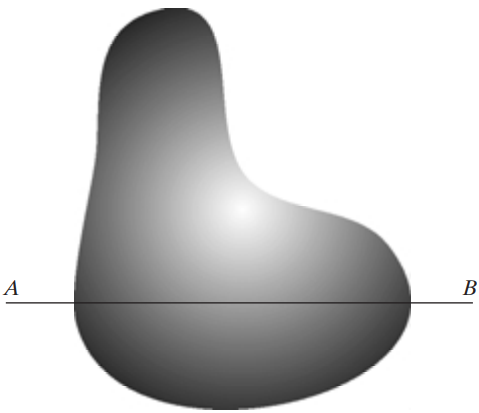
\includegraphics[width=0.3\textwidth]{Imagenes/Digitalizacion_1.png}
	\caption{Entrada continua al sistema.}
	\label{fig:disc1}
\end{figure}

Por lo tanto, se deben tomar coordenadas finitas, por ejemplo, aquellas que se encuentran sobre la recta AB, y asignarle a cada una un valor dado de amplitud. En la Figura~(\ref{fig:disc2}) se observa como una recta continua paralela al eje $x$ (horizontal), la cual posee ciertas variaciones aleatorias dadas por el ruido existente, es dividida en una cierta cantidad de posiciones equiespaciadas (discretización), marcadas con cuadrados blancos sobre la curva, asigandoles un nivel específico en la escala de grises (cuantización), marcado con una linea negra por la izquierda de dicha escala.
\begin{figure}[H]
\centering
	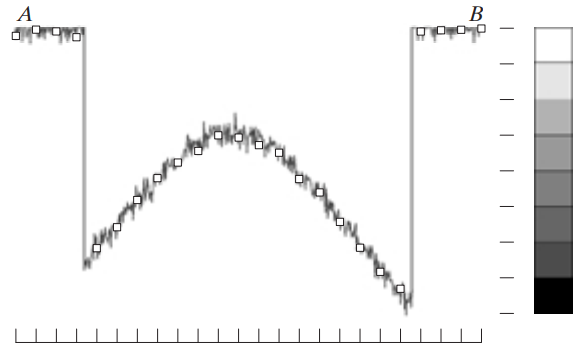
\includegraphics[width=0.5\textwidth]{Imagenes/Digitalizacion_2.png}
	\caption{Amplitud de la escala de grises en la recta AB y muestreo de valores.}
	\label{fig:disc2}
\end{figure}

Realizando el mismo proceso para todos los niveles de discretización en el eje $y$ (vertical), se obtiene finalmente una imagen digitalizada, la cual se la compara a continuación con la original \cite{ref:digit1}.
\begin{figure}[H]
\centering
	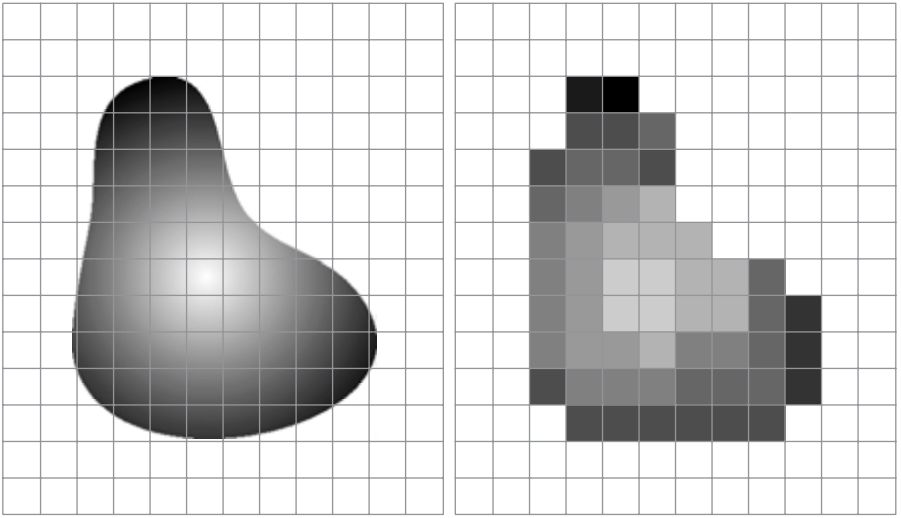
\includegraphics[width=0.5\textwidth]{Imagenes/Digitalizacion_3.png}
	\caption{Imagen original comparada con la imagen digitalizada a procesar.}
	\label{fig:disc3}
\end{figure}

\textcolor{red}{
\begin{itemize}
	%\item Descripción de las líneas de investigación (con referencias).
	\item Descripción de los conceptos más importantes de cada una.
	\item Análisis propio de lo presentado.
	\item Simulaciones de lo más relevante (códigos como apéndice)
	\item Elección del camino y justificación.
\end{itemize}
}

	De esta forma, este trabajo se centra en procesos de medio nivel. Dicha definición es muy amplia, por lo cual es necesario acotar dicho camino. Es por ello que se decidió centralizarse en el seguimiento de objetos en imagenes en movimiento.
	
	\textcolor{blue}{Escribí una brevísima descripción de lo que se va a hacer. Profundizar y escribir el objetivo final. Justificar elección.}

\section{Aportes}
\textcolor{red}{
\begin{itemize}
	\item Descripción y análisis de lo original producido por el grupo.
	\item Simulaciones que justifiquen las ideas, y que prueben su originalidad.
	\item Análisis de resultados
\end{itemize}
}

\section{Desarrollo}
\textcolor{red}{
\begin{itemize}
	\item Viabilidad, caminos alternativos.
	\item Proceso de implementación
	\item Documentación de los resultados: Resumen de lo más relevante, demos y programas van al apéndice.
	\item Evaluación y conclusiones del desarrollo.
\end{itemize}
}

\begin{thebibliography}{9}
\bibitem{ref:intro1}
R. C. Gonzalez, R. E. Woods and S. L. Eddins. \textit{Digital Image Processing Using MATLAB}. Prentice Hall, 2nd ed, 2002, pp. 2-3.

\bibitem{ref:digit1}
R. C. Gonzalez, R. E. Woods and S. L. Eddins. \textit{Digital Image Processing Using MATLAB}. Prentice Hall, 2nd ed, 2002, pp. 52-54.
\end{thebibliography}


\end{document}